\section{Chemical intuitions}\label{sec:chemical-intuitions} % (fold)
Huet's original insight was that we can describe a location in a tree
via a pair consisting of a context (a tree with a hole in it) and a
tree (think of it as a subtree to be plugged into the hole).
McBride's analysis of the zipper begins by with the brilliant
observation that contexts can be calculated for a wide range of data
types, namely those expressible as differentiable functors. The two
ideas in combination give a calculus for computing locations in data
structures.

\begin{figure}
  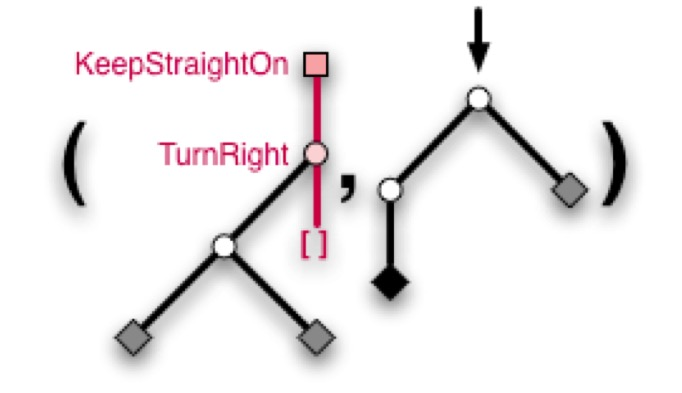
\includegraphics[width=\linewidth]{ZipperFigure1.jpg}
  \caption{Tree location}
  \label{fig:tree-location}
\end{figure}

Meanwhile, Milner proposed the radical idea of turning functions into
processes by liberating computational interaction from textual
juxtaposition \cite{DBLP:journals/mscs/Milner92}. In the
$\lambda$-calculus $\beta$-reduction only happens when an abstraction
is applied to a term. That is, when they are \emph{placed next to each
  other in a reduction context}. The $\pi$-calculus refines this idea,
first by providing a symmetric, associative term constructor, namely
parallel composition, that allows terms to freely mix (hence Berry and
Boudol's intuitions regarding chemical abstract machines
\cite{DBLP:journals/tcs/BerryB92} were so apt a semantic framework for
understanding Milner's calculus).

Having liberated terms from mere juxtaposition, Milner needed to
provide a way for data exchange and computational evolution to
occur. This is accomplished in the $\pi$-calculus by reifying the site
of interaction in the form of a channel. These freer, more mobile
computations are called processes, as opposed to the
$\lambda$-calculus' \emph{functions}.

Milner's calculus, however, suffers a flaw in that a theory of names
must simultaneously be countably infinite, enjoy an effective
equality, and \emph{have no internal structure}. Taking all three
together makes them unrealizable in modern computers. Meredith's
reflective, higher-order calculus (rho-calculus, for short) remedies
the situation by making channels be \emph{quoted processes}, thus
supplying internal structure and higher order capabilities in a single
feature \cite{DBLP:journals/entcs/MeredithR05}.

In a semantic setting the shift from $\pi$ to rho-calculus can be seen
in terms of a domain equation and its fixpoint.

\begin{mathpar}
  P[X] = 1 + (X \times P[X]) + (X \times X) \times P[X] + (P[X] \times P[X]) + X \\
  R = P[R]
\end{mathpar}

The domain equation is indeed a differentiable functor, and this we
can provide a notion of location in a process term, that is $L[X] := P[X] \times \partial P[X]$. This allows us to reconcile channels as
locations in a computation.

\begin{mathpar}
  LP = P[P[LP] \times \partial P[LP]]
\end{mathpar}

Your author wrote down this equation in 2008 and could not find a
calculus that solved it until 2018. The calculus presented below is
the solution he discovered in 2018.

The key idea returns again to \emph{chemical} intuitions. The first
step is to introduction a \emph{catalyst} that must be present in
order for redexes to reduce. In the rho-calculus a term of the form
$\binpar{\prefix{x}{y}{P}}{\outputp{x}{Q}}$ would ordinarily reduce to
a term of the form $P{\substn{\quotep{Q}}{y}}$. In the space calculus
(from outer space!) that term is inert. It must have a catalyst of the
form $\mathsf{COMM}(K)$ mixed in,
i.e. $\binpar{\mathsf{COMM}(K)}{\binpar{\prefix{x}{y}{P}}{\outputp{x}{Q}}}$,
before it can reduce. This feature makes the space calculus (from
outer space!) the only process calculus genuinely requiring a ternary
interaction rule.

The catalyst is necessary because names are now not merely quoted
processes, but pairs of contexts and processes,
$\spacen{K}{Q}$. Additionally, while the rho-calculus leaves unbound
terms of the form $\dropn{\quotep{P}}$ inert, the space calculus
(don't worry i'm not going to keep saying ``from outer space!'' over
and over again) allows these terms to evolve to produce catalysts
(thus allowing for autocatalysis). Foreshadowing what's to come, we'll see a new reduction rule of the form

\begin{mathpar}
  \inferrule* [] {}{\binpar{\mathsf{U}(x)}{\spacen{K}{Q}} \red \binpar{\mathsf{COMM}(K)}{\outputp{x}{Q}}}
\end{mathpar}

\section{Contextual interlude}\label{sec:contextual-interlude} % (fold)
There is a natural half-way point on the way to these ideas. There is
an extension of the rho-calculus where the $\mathsf{COMM}$ rule is
parameterized by a context. In the original rho-calculus, we have terms of the form

\begin{mathpar}
  \inferrule* [lab=process] {} {P, Q \bc \pzero \;\bm\; \mathsf{for}(y \leftarrow x )P \;\bm\; x\mathsf{!}(Q) \;\bm\;
  P\mathsf{|}Q \;\bm\; \mathsf{*}x }
  \and
  \inferrule* [lab=name] {} {x, y \bc \quotep{P} }
\end{mathpar}

And a core reduction rule of the form

\begin{mathpar}
  \inferrule* [lab=Comm] {x_{t} \;\nameeq\; x_{s}} {\mathsf{for}( y \leftarrow x_{t} )P \;\mathsf{|}\; x_{s}!(Q)
    \red P\substn{\quotep{Q}}{y}} \\
\end{mathpar}

We can contemplate a parameterization of this rule in terms of a context parameter $K$.

\begin{mathpar}
  \inferrule* [lab=Comm(K)] {x_{t} \;\nameeq\; x_{s}} {\mathsf{for}( y \leftarrow x_{t} )P \;\mathsf{|}\; x_{s}!(Q)
    \red P\substn{\quotep{K[Q]}}{y}} \\
\end{mathpar}

This choice allows for multiple instances of the rule using different
contexts, such as $K_{1}$ and $K_{2}$. Thus, affording us a notion of
composition of calculi, say $\langle \Proc, \mathsf{COMM}(K_{1}) \rangle$, and $\langle \Proc, \mathsf{COMM}(K_{2}) \rangle$ through the composition of contexts, yielding $\langle \Proc, \mathsf{COMM}(K_{2} \circ K_{1}) \rangle$. Where we use $\Proc$ for the set of terms freely generated by the grammar.

This idea is useful for modeling ``impedance matching'' of behaviors
at different layers or different scales. For example, the
$\mathsf{TCP}$ protocol is at a different layer than the
$\mathsf{HTTP}$ protocol. Yet, it is common for applications to
utilize both protocols. We can use the contexts to factor all the
boilerplate protocol translation from one layer to the other. A
similar sort of application can be found in modeling chemical versus
biochemical versus biological level phenomena.

As useful as the technique is, it is fixed. It doesn't allow for
programmable contexts. The space calculus can be thought of as the
next natural step in this line of reasoning, affording a dynamic,
programmable factorization of a contextual interface.
